\documentclass[12pt,twosides]{book}
\usepackage{amsmath}
\usepackage{graphicx}
\usepackage{color}
\usepackage{setspace}
\doublespacing
\begin{document}

\section{abstract}

One of the most basic open questions in physics today concerns the nature of dark matter. There has been strong observational evidence for the existence of dark matter for nearly eighty years, yet we still know little about dark matter, despite the fact that it composes $26.8\%$ of our universe. One leading candidate for dark matter is the axion, a light pseudoscalar particle. Searches for the axion have been experimentally challenging, as the axion's coupling to ordinary matter is very weak. One technique that is extremely sensitive to dark matter axions is the method of resonant detection using microwave cavities and the Primakoff effect to convert axions to photons in a strong magnetic field. This method has been applied successfully to rule out models of axions from 1.9 to 3.5 $\mu$eV. However, prior to this work , the technique had not been applied to look for axions of higher mass in the 0.1 to 1 $meV$ range. It is interesting to search for axions in this mass range because it is complementary to current axion microwave cavity searches, because there are several hints that the favored axion mass is in this range, and because the recent BICEP results constrain the axion mass in a simple cosmological history to be within that region. We present here the first microwave cavity search for dark matter axion-like particles in this region. By tuning a cryogenically cooled cavity and measuring the $TM_{020}$ mode in a 7 Tesla background magnetic field, we look for axion-like particles (if they form part of the dark matter) that transform to photons via the Primakoff effect. When the photon frequency equals the microwave cavity resonant frequency, the signal power is enhanced. Cryogenic amplifiers and a low noise receiver chain allow us to reduce our background from thermal noise. In our experiment, we ran for four months and swept the microwave cavity resonant frequency from 33.9 to 34.5 GHz, corresponding to an axion mass of 140.2  to 142.7 $\mu$eV and were able to exclude an ALP to two photon coupling of $g_{a\gamma\gamma} < 8\times10^{-11}$ 1/GeV, marginally improving on the CAST limit. We are also able to set limits on hidden photon coupling to matter if these vector bosons are responsible for dark matter. As with the first generation of microwave cavity experiments that searched for axions in the lower mass region, there are several technical challenges that must be solved in order to reach the sensitivity to observe or exclude canonical axion models. However, as we do not know where the axion mass is it is valuable to develop experiments and techniques to search for them in their entire possible mass range. If observed, axion (and ALP) dark matter would not only be an important advance in our knowledge of dark matter but also give us clues about processes at high energy scales inaccessible by other methods.

\tableofcontents
\section{Acknowledgments}

\chapter{Background and Motivation}

%\subsection{The Nature of Dark Matter, Physics at High Energy Scales}

One of the most basic open questions in physics today concerns the nature of dark matter. Nearly eighty years ago, strong observational evidence was presented that non-luminous, gravitationally interacting matter exists \cite{zwicky37}; since then the existence of matter that does not interact electromagnetically has been shown, with strong evidence in the rotation curves of spiral galaxies \cite{rubin80}, and precision measurements of the Cosmic Microwave Background can measure the dark matter density in our universe to be 23$\%$ \cite{planck14}. However, to date we know little more than the fact that this dark matter is most likely a stable, neutral particle that is non-relativistic and non-baryonic [NEEDSREF]\footnote{although dark matter could be caused by modifications to gravity}. There are several strongly motivated candidates for dark matter; the three most promising today are sterile neutrinos \cite{kusenko09}, Weakly Interacting Massive Particles (WIMPs) [NEEDSREF], and axions. 

WIMPs have historically been the most popular dark matter candidate; they are particles that have weak scale cross-sections with ordinary matter. The theoretical support for WIMPs comes from Supersymmetric theories (SUSY), which solves what is known as the gauge hierarchy problem, or the fact that the Higgs mass is quadratically divergent. By introducing partners for all the known partners with opposite spin-statistics, SUSY solves this divergence problem. The lightest SUSY particle, the neutralino, would be a WIMP. Various experiments have searched for WIMPs, either directly through the recoil of nuclei when WIMPs strike them \cite{lux14}, indirectly through their annihilation with each other in the galaxy \cite{slatyer09}, as well as searches in colliders \cite{rajaraman11}. The null results from these experiments suggest that it is worthwhile investigating all dark matter candidates. Moreover, dark matter could be formed from any or all of these particles. This work focuses on a dark matter axion-like particle search. Axion-like particles (ALPs) are light bosons that have similar interactions and properties as the axion, but do not arise from the same theory.

The work done as part of the Yale Microwave Cavity Experiment (YMCE) was a search for dark matter pseudoscalars that couple to two photons, also known axion-like particles (ALPs). This project is part of YMCE's work in constraining exotic particles in the 140 $\mu$eV mass region using cryogenically cooled microwave cavities, with previous projects being a search for dark matter scalars, and one looking for photon regeneration due to hidden photons. This mass region is so far unexplored by other microwave cavity experiments, as it is more challenging to reach the sensitivities needed to detect the theorized axion.

This work describes the dark matter search; the design of the cavity, operation of the experiment, and measurements taken. The remainder of this chapter discusses the motivation for axion (and ALP) dark matter in more detail. Chapter 2 describes the technique of using microwave cavities, while Chapter 3 provides some background on astrophysics and cosmology necessary for understanding the current parameter space. Chapter 4 describes the experiment, while Chapters 5, 6, and 7 focus on the microwave cavity design and data analysis, which I worked on. This includes simulations of the cavity coupling and itsform factor, tuning, and Q response at cryogenic temperatures (Chapter 5), the construction of a data analysis pipeline and determining an exclusion limit (Chapter 6), and work on the hardware automation for the experiment (Chapter 7).

\section{How does the axion come/ and why is it a good dark matter candidate?}

We briefly review motivations for the axion and axion-like particles (ALPs) as a dark matter candidate. For a more comprehensive discussion see \cite{hewett12}, \cite{arias12}, and \cite{kim87}. 

\subsection{strong CP problem}

The motivation for axions, or QCD axions, is very strong. The axion arises from a mechanism introduced to explain the puzzling fact that parity and time violation are not observed in the theory of strong interactions, Quantum Chromodynamics (QCD). This is odd, as there is a term in the QCD Lagrangian that is explicitly P- and T- violating:

\begin{align*}
\mathcal{L} = \bar \theta g^2 G \tilde G
\end{align*}

where $\bar \theta$ is a phase between $-\pi$ and $\pi$, G is the gluon field tensor and $\tilde G$ is the dual, or $G_{ab} = \epsilon-{abcd} G^{cd}$. To see that it is parity and time violating, construct the color electric and magnetic field equivalents from the tensor: for the electromagnetic field tensor $FF = E^2 -B^2$ and $F\tilde F = E\dot B$. Therefore for the gluon field tensor, $G\tilde G = E_a \dot B_a$. Under a parity transformation ($x \rightarrow -x$), $E \rightarrow E$ and $B \rightarrow -B$. Under a time transformation, $
E \rightarrow E$ and $B \rightarrow -B$.  Therefore the product $E\dot B$ is not symmetric under parity and time reversal. By the CPT theorem [NEEDSREF], T-violation is equivalent to CP-violation.

\footnote{We note that the reason the equivalent CP violating term in QED does not arise $F\tilde F$ is because it is a total four-divergence. This means, for fields that are vanishing small as you approach spatial infinity, that the term goes to zero when integrating the Lagrangian. Because the gluon fields are self-interacting (you can equivalently say QCD is non-abelian) the term $G \tilde G$ is not zero as you go to infinity, and so the four divergence has a finite effect.}

 From this CP violating term we should see a neutron electric dipole moment [NEEDSREF] [NEEDSPIC]. However measurements of the neutron EDM have been consistent with zero, placing an upper boud on $\bar \theta < 10^{-10}$.

Although there is a free parameter, $\bar \theta$ in this P, T (or CP- if you believe in the CPT Theorem) violating term that can be set to zero, this constitutes a fine tuning problem as the observable $\bar \theta$ is the sum of two independent terms from two different sectors, which should not a priori cancel each other.

\begin{align*}
\bar \theta = \theta + \text{arg det} \mathcal{M}
\end{align*}

The physical meaning of these terms is that $\theta$ is the density of instantons. Instantons are tunneling events that occur being different QCD vacua. We know that QCD has a non-trivial vacua because the introduction of such a vacua solves the $U(1)_A$ problem, which is the question of why the $\eta'$ is not degenerate with the pion mass \cite{thooft76}. The problem is a question of symmetry breaking - [NEEDSEXPLANATION]. $\mathcal{M}$ is the quark mass matrix: $\text{arg det} \mathcal{M} = m_um_dm_s$ the product of the quark masses when real. If there is a massless quark, the value above is undefined and $\bar \theta$ is also undefined. However, we believe there is evidence that the lightest quark, the up, is not massless and has mass between 0.3-0.7 MeV [NEEDSREF].

 This "strong CP problem", or the fine tuning problem of why $\bar \theta$ is less than a billionth of a radian when there is no reason to believe it should be so small, can be solved by introducing a new global, chiral symmetry, as proposed by Peccei and Quinn in 1977 \cite{peccei77}. The spontaneous breaking of this symmetry at some energy scale $f_a$ (that the symmetry must be broken is due to the non-vanishing quark masses) introduces the axion as the resulting massless Goldstone boson. Due to a chiral anomaly with QCD, or to rephrase due to instanton effects, the axion experiences a potential, which causes it to acquire a mass proportional to the energy scale of QCD, $\Lambda_{QCD}$ and inversely proportional to the energy scale of the symmetry breaking $f_a$ \cite{weinberg78}, \cite{wilczek78}. The role of anomalies is widespread in physics; a chiral anomaly with electromagnetic fields solves the U(1) problem, which is the question of why the $\eta'$ is not degenerate with the pion mass. It is due to anomalies that this occurs. For more comprehensive treatment of anomalies, see \cite{bardeen07}. The axion coupling constant to matter ends up also being inversely proportional to $f_a$, so the mass and coupling constant of the axion are directly proportional. The axion coupling to gluons implies a generic coupling to photons, through mixing with the pion; although there is some model dependence for the coupling and it can be set to zero, this represents another fine tuning problem.

[NEEDSPIC] of axion to gluon coupling, axion to pion coupling

The term axion-like particles (ALPs) describes bosons that, like the axion, acquire a mass through some explicit symmetry breaking of a new symmetry, although not necessarily due to an anomalous interaction with QCD. Familons and majorons are two such examples of ALPs \cite{kim87}, but they arise generically in string theories  and extensions to the standard model,\cite{masso06}, \cite{hewett12}, \cite{arias12} as the mechanism of an additional U(1) symmetry is a minimal extension, and anomalies must often take place to cancel divergences. For ALPs, the coupling and mass are no longer necessarily connected, so there are two free parameters to their theory. However, the idea of a light, spinless, neutral, chargeless boson is common for both axions and ALPs.

\subsection{Models of the axion}

The first model of the axion came from introducing the new symmetry through two Higgs doublets, as proposed by Peccei and Quinn. The two doublets, $\lambda_1$ and $\lambda_2$ combine to have a non-zero vacuum expectation value. The phase of the vacuum expectation value is the axion; by current algebra techniques that mass of the axion can be computed to be 

\begin{align*}
m_a = \frac{Nm_\pi f_\pi}{v_F}\frac{\sqrt{z}}{1+z}(\frac{1}{x}+x) = (23 \text{keV})(\frac{1}{x}+x)
\end{align*}

for $ x = <\lambda_1>/<\lambda_2>$ is the ratio of the vacuum expectation values of the doublets and $z = m_u/m_d$ is the ratio of the up and down quark masses.

This Peccei-Quinn-Weinberg-Wilczek axion was predicted to have a mass of some keV, but was ruled out in reactor and accelerator experiments \cite{crystalball90} [NEEDSREF].

Simple extensions to the Peccei Quinn mechanism modified the energy scale of the symmetry breaking, decoupling it from the electroweweak scale, and allowing the axion mass to be much lighter. The Dine, Fischler, Srednicki, Zhitniskii model (DFSZ) \cite{dine81},\cite{zhitniskii81}, adds a single heavy scalar in addition to the Higgs doublets introduced before. 

The mass of the axion is then calculated to be:

\begin{align*}
m_a = \frac{f_\pi}{f_a} m_\pi N \frac{\sqrt{z}}{1+z}
\end{align*}

For $z= 0.56$, $f_\pi = 93 \text{ MeV}$, and $m_\pi = 135\text{ MeV}$, $m_a \approx \frac{10^7\text{GeV}}{f_a}eV$.

Another model, the Kim, Vainshtein, Shiman, Zakharov model \cite{kim79},\cite{shifman80}, extends the Peccei Quinn mechanism by introducing a new heavy quark and complex scalar field, as well as a discrete symmetry. The axion then couples directly to this heavy quark and through the quark, to ordinary matter. The axion mass is then:

\begin{align*}
m_a = \frac{\sqrt{z}}{1+z}m_\pi\frac{f_\pi}{f_a}
\end{align*}

and the coupling to two photons is:

\begin{align*}
g_{a\gamma\gamma}^{KSVZ} &= \frac{\alpha}{2\pi f_a}(\frac{E}{N}-\frac{2}{3}\frac{4+z}{1+z}) 
\\ &= 1.93\times10^{-15}\text{GeV}^{-1}(\frac{E}{N}-\frac{2}{3}\frac{4+z}{1+z})(\frac{m_a}{10^{-5}\text{eV}})
\end{align*}

In conclusion, for the two photon interaction for which $\mathcal{L} = g_{a\gamma\gamma}E\dot B a$, the coupling is

\begin{align*}
g_{a\gamma\gamma} &= -\frac{3\alpha}{8\pi f_a}\xi = - \frac{m_a/\text{eV}}{0.69\times10^{10}\text{ GeV}}\xi 
\\ \xi &= \frac{4}{3}(\frac{E}{N} - 1.92 \pm 0.08)
\end{align*}

$E/N$ is the ratio of the color to electromagnetic anomalies. For the DFSZ mode it is 8/3, for the KVSZ model it is 0. It cannot be guaranteed that $E/N$ does not equal 2, however, in which case the coupling to photons would be severely suppressed.


\section{Detecting axions}

Astrophysical arguments can constrain the axion mass severely. The requirement is that axions, which can produced in the cores of stars and act as an additional energy loss channel, have couplings lower than those which would produce a conflict with observation. The limits on the coupling strength to photons for globular clusters and the limit on the coupling strength to nucleons in the case of supernova SN1987A can be translated into limits on the axion mass of $m_a \leq 10^{-2} \text{eV}$ or $f_a \geq 10^9\text{GeV}$ \cite{raffelt08}.

I briefly review the techniques used to search for axions:

\begin{description}

\item \textbf{Solar axions} \hfill \\

Here one uses the Primakoff effect to search for axions produced in the sun due to the strong electric and magnetic fields in the plasma. By aiming a dipole magnet at the sun, the axions streaming from the sun can reconvert into photons (x-rays) and then be detected. The main experiment here is CAST \cite{cast11}, which has begun to edge out the globular cluster limit although not completely.  As \cite{raffelt08} notes, because the massive axions are converting to massless photons, there is a large momentum mismatch. The massive axion as momentum $k_a = (\omega^2 - m_a^2)^{1/2}$ while the photon has momentum $k_\gamma = \omega$. The difference is $q = k_\gamma - k_a \approx m_a^2/2\omega$ for $m_a \ll \omega$, so the length over which one can coherently detect a signal is limited, so conversion is a function of length.

\item{Bragg diffraction}
Another experiment used the electric fields of crystals to convert 

\item{Vacuum Birefringence}

\item{Rydberg Atoms}

\item{Photon Regeneration}


\item{Mossbauer Absorption}

\item{Oscillating EDMs, Dish Antennas}

\item{RF cavity}

While in the helioscopes the conversion was proportional to the length of the detector, for axions traveling along the magnetic field, for axion to photon transitions in the presence of a background magnetic field with high-Q cavities, the conversion probability depends on the overalp of the magnetic field and the electric field of the cavity mode, so thus the volume.

\end{description}

\begin{figure}
\centering
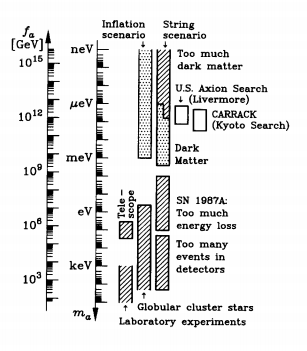
\includegraphics[width=0.6\textwidth]{1dexclusionlimit}
\caption{Constraints on the axion mass (and thus energy scale) from \cite{raffelt80}. Striped lines are constraints; blank are projected constraints; and dotted are dependent on the cosmological history of the axion.}
\end{figure}

\begin{figure}
\centering
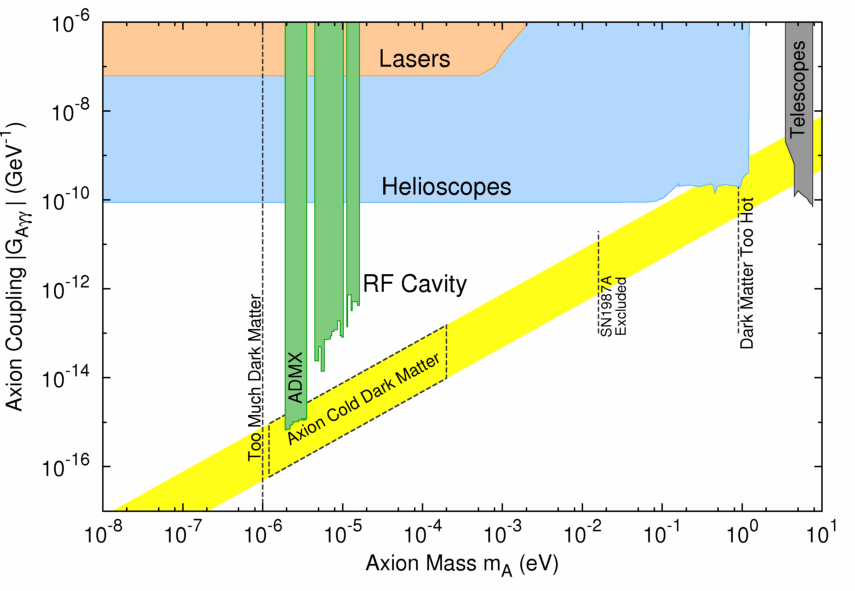
\includegraphics[width=\textwidth]{2dexclusionplot}
\caption{Summary of the ALP and axion parameter space. In yellow are shown the axion model bounds. ADMX, in green, and their experimental limits begin to constrain the axion models. Helioscopes, led by CAST, and their limits are shown in blue; photon regeneration expts labeled as Lasers exclude the upper right region but do not assume anything about dark matter so are more rigorous. The dashed line labeled SN1987A is the exclusion on the axion mass extrapolated from the observation of neutrino events from SN1987A.}
\end{figure}

\section{The Primakoff Effect}

We have referred to the Primakoff effect several times; this is the axion-two photon interaction that most axion experiments use and that is capitalized on in this work. To see how this occurs, we write the effective Lagrangian for the ALP to gluon coupling once more:

\begin{align*}
\mathcal{L} = \bar \theta g^2 G \tilde G = \frac{a}{f_a} g^2 G \tilde G
\end{align*}

This hides the fact that there is a triangle loop causing a Yukawa coupling between the axion and the intermediate fermion which couples to the gluons. Either this fermion is a heavy quark (as in the KSVZ) model, or an ordinary fermion.

The gluons can create quark-anti-quark pairs, with the pion being the lightest example. One can think of this axion-pion mixing as the effect that generates the axion mass. The pions can then decay into two photons via the Primakoff effect, which itself has a triangle loop anomaly, and this is how the axion interacts with two photons.

\section{How axions are produced as dark matter}

So far we have explained how axions in particular can be produced as the result of a new symmetry having an anomaly with QCD. Now let us consider what happens during the evolution of the axion. The potential that the axion feels is a function both of $\theta$ and T, the temperature. 

\begin{figure}
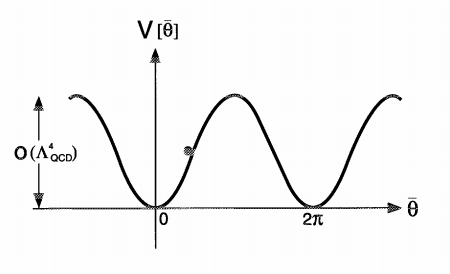
\includegraphics[width=0.6\textwidth]{vthetavstheta}
\end{figure}


\begin{figure}
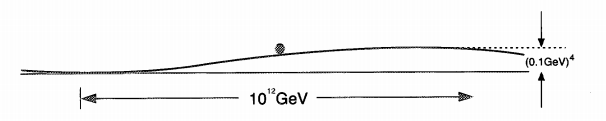
\includegraphics[width=0.6\textwidth]{axionpotential}
\caption{From \cite{kim95}; shows how slight the axion potential is.}
\end{figure}

Imagine this potential being stretched out in space, as is happening through the expansion of the universe. When the expansion slows down sufficiently so that $H \simto m_a$, the axion begins to oscillate. Because the lifetime of the axion is longer than the age of the universe, the oscillations do not die out, but the amplitude of the oscillations is decreased by the expansion of the universe. Discussion taken from Kim's "Axionic Extensions of the Standard Model".

The energy scale in relation to the energy scale of inflation leads to different predictions. If the mass turns on before inflation sets in, that leads to a lower bound on the axion mass, as otherwise they would be overproduced. Usually this limit is set at $10^{-6}$ eV. However extrapolating from the high energy scales and today's energies leaves a lot of room for uncertainty so this lower limit bound is subject to debate. The recent BICEP results \cite{bicep14}, although they need to be verified, set the inflation scale at $10^16$ GeV and the Hubble scale at which this happened at $10^14$ GeV, by the observation of B mode polarization in the CMB. Almost immediately after the results were reported, Ref \cite{visinelli14} showed that this would exclude the simplest cosmological model of the axion except for the mass range 72 $\mu$eV to 1meV. The reason is something called isocurvature perturbations, as idiscussed in Ref \cite{fox04}. The BICEP results at the time of writing are coming under scrutiny and don't seem to be holding up, very well - so an independent verification within a year will show whether or not to go forward this limits.

\section{Isocurvature Perturbations}

...

There are also other non-thermal mechanism to produce the axion. 
\begin{description}
\item Cosmics strings

\item Domain Walls

\end{description}


\section{Supernova Limit}

We make a note here about the supernova limit and how it was achieved. The limit is $6 \times 10^{-11}$ 1/GeV; better than the limits produced by this experiment. However, we appeal to systematic uncertainties in the understanding of supernova physics.



\subsection{Searching for axions in the lab}

From the theory and constraints we see that axions (and ALPs) can live anywhere from 1 picoeV (the Planck scale) to 1 meV. Astrophysical bounds limit the upper mass range; there are some cosomological arguments limiting the axion mass to $1 \mu$eV and greater. In this range, From the Primakoff effect, an axion converting to a photon in the presence of another photon will give the resulting photon its energy. If the axion is non-relativistic, the photon energy will be the axion rest mass (which for an axion between 1 $\mu$eV and 1 meV translates to a frequency of 700 MHz to 300 GHz). Thus the axion would produce a microwave photon. Using microwave cavities to compensate for the strong momentum mis-match and also to enhance the sgnal power, and also using strong magentic fields, with the axion dark matter source one can reach the axion model band with some technical leaps.

The work in this thesis describes a search for dark matter axion-like particles, using a cryogenically cooled microwave cavity in a strong magnetic field.


\bibliographystyle{plain}
\bibliography{thesisbib}
\end{document}